\documentclass[preprint,12pt,aps,pra,showkeys,amsmath,amssymb,superscriptaddress,floatfix]{revtex4-2}
\usepackage[T1]{fontenc}
\usepackage[utf8]{inputenc}
\usepackage{amsmath,amssymb,amsthm,mathtools,mathrsfs}
\usepackage{microtype,booktabs,enumitem}
\usepackage{xcolor,tikz,etoolbox}
\usepackage[skins,breakable]{tcolorbox}
\usepackage{needspace}
% Keep diagram geometry independent of REVTeX preprint body spacing.
\AtBeginEnvironment{tikzpicture}{\linespread{1}\selectfont}
\usetikzlibrary{arrows.meta,positioning,calc,fit,decorations.pathreplacing}
\usepackage{graphicx}
\usepackage{hyperref}

\definecolor{MMBlue}{RGB}{0,82,155}
\definecolor{MMOrange}{RGB}{200,80,0}
\tikzset{
 mmnode/.style={draw=MMBlue,rounded corners=2pt,fill=MMBlue!4,align=left,execute at begin node={\raggedright},text width=5cm,font=\fontsize{10}{12}\selectfont,inner sep=6pt},
 mmimport/.style={mmnode,draw=black!65,fill=black!4},
 mmcandidate/.style={mmnode,draw=MMOrange,dashed,fill=MMOrange!5},
 mmrejected/.style={mmnode,draw=black,densely dotted,fill=black!8},
 mmproof/.style={->,thick,MMBlue},
 mmflow/.style={->,semithick,black!70},
 mmrepair/.style={->,dashed,thick,MMOrange},
 mmcandidatearrow/.style={->,dashed,semithick,MMOrange},
 mmnote/.style={font=\scriptsize,fill=white,inner sep=2pt,align=center}}

\usepackage[section]{placeins}
\setlength{\emergencystretch}{3em}
\setlist{itemsep=3pt,topsep=4pt}
\newtheorem{theorem}{Theorem}[section]
\newtheorem{proposition}[theorem]{Proposition}
\newtheorem{lemma}[theorem]{Lemma}
\newtheorem{corollary}[theorem]{Corollary}
\theoremstyle{definition}
\newtheorem{definition}[theorem]{Definition}
\newtheorem{example}[theorem]{Example}
\theoremstyle{remark}
\newtheorem{remark}[theorem]{Remark}
% Avoid isolated statement headings and single-line paragraph fragments.
\BeforeBeginEnvironment{theorem}{\Needspace{6\baselineskip}}
\BeforeBeginEnvironment{definition}{\Needspace{5\baselineskip}}
\BeforeBeginEnvironment{proposition}{\Needspace{5\baselineskip}}
\BeforeBeginEnvironment{lemma}{\Needspace{5\baselineskip}}
\BeforeBeginEnvironment{corollary}{\Needspace{5\baselineskip}}
\clubpenalty=5000
\widowpenalty=5000
\newcommand{\R}{\mathbb R}\newcommand{\Z}{\mathbb Z}\newcommand{\N}{\mathbb N}
\newcommand{\Pa}{\operatorname{Pa}}\newcommand{\Desc}{\operatorname{Desc}}
\newcommand{\cl}{\operatorname{cl}}\newcommand{\cost}{\operatorname{cost}}
\newcommand{\status}{\operatorname{status}}
% Faculty cards: a visual rail groups the five faculties within one agent.
% The rail has no arrowhead and does not represent a proof dependency.
\newcommand{\mmfacultybadge}[1]{%
 \node[circle,draw=MMBlue,line width=1pt,fill=white,
 minimum size=7mm,inner sep=0pt,font=\sffamily\small\bfseries,text=MMBlue]
 at ([xshift=15pt,yshift=-15pt]frame.north west) {#1};}
\newcommand{\mmfacultyrail}{%
 \draw[MMBlue!80,line width=1pt]
 ([xshift=15pt,yshift=2pt]frame.north west)--
 ([xshift=15pt,yshift=-2pt]frame.south west);}
\newtcolorbox{mmfacultybox}[2]{enhanced,breakable,
 colback=MMBlue!4,colframe=MMBlue!4,boxrule=0pt,arc=3pt,
 left=39pt,right=9pt,top=4pt,bottom=4pt,
 before skip=2pt,after skip=2pt,
 fontupper=\small\linespread{1.1}\selectfont,
 overlay unbroken={\mmfacultyrail\mmfacultybadge{#1}},
 overlay first={\mmfacultyrail\mmfacultybadge{#1}},
 overlay middle={\mmfacultyrail},overlay last={\mmfacultyrail}}
\newcommand{\mmfaculty}[3]{%
 \begin{mmfacultybox}{#1}{#2}
 {\sffamily\bfseries\color{MMBlue}#2}\par\smallskip #3
 \end{mmfacultybox}}
\newcommand{\agent}[9]{%
 \Needspace{8\baselineskip}
 \subsubsection{#1}
 \noindent\textbf{Object.} #2\par
 \noindent\textbf{Role.} #3\par\smallskip
 \mmfaculty{E}{Ego}{#4}
 \mmfaculty{M}{Memory}{#5}
 \mmfaculty{I}{Intellect}{#6}
 \mmfaculty{S}{Sense}{#7}
 \mmfaculty{A}{Action}{#8}
 \smallskip\noindent #9\par}

\usepackage{longtable,array,calc}
\providecommand{\tightlist}{\setlength{\itemsep}{2pt}\setlength{\parskip}{0pt}}
\makeatletter
\def\frontmatter@abstract@produce{\par\addvspace{\frontmatter@preabstractspace}%
\begingroup\prep@absbox\unvbox\absbox\post@absbox\endgroup
\addvspace{\frontmatter@postabstractspace}}
\makeatother
\newcommand{\field}[2]{\par\smallskip\noindent\textbf{#1.} #2\par}
\setlength{\emergencystretch}{5em}
\AtBeginEnvironment{verbatim}{\small\linespread{1.0}\selectfont}


\hypersetup{colorlinks=true,linkcolor=MMBlue,urlcolor=MMBlue,pdfauthor={Dibakar Sigdel}}

\begin{document}

\title{Existence and Uniqueness for the Weak Poisson Problem\\[4pt]\large An End-to-End Meta-Math Walkthrough}

\author{Dibakar Sigdel}

\affiliation{Mindverse Computing LLC, Lynnwood, WA 98087, USA}

\date{October 2026}

\begin{abstract}

The gradient form becomes an inner product once a Poincaré estimate
controls the missing \(L^2\) part. Riesz representation then constructs
the weak solution directly. The report presents the target theorem,
declared imports, a dependency graph, five-faculty node contracts, a
continuous proof, a worked example, and a hypothesis-repair audit. It is
an authored mathematical exposition, not a deployed-agent transcript or
a formal proof-assistant certificate.

\end{abstract}\maketitle\linespread{1.12}\selectfont

\noindent\textbf{PDE-02 / Partial Differential Equations / Report v1}

\section{Target and import contract}

\begin{theorem}

Let \(\Omega\subset\mathbb R^d\) be nonempty, bounded, and open, and let
real \(f\in L^2(\Omega)\). Prove there is a unique
\(u\in H_0^1(\Omega)\) such that
\(\int_\Omega\nabla u\cdot\nabla v=\int_\Omega fv\) for every
\(v\in H_0^1(\Omega)\). If \(\Omega\) lies inside a cube of side \(L\),
prove \(\|\nabla u\|_2\le L\|f\|_2\). This is a weak solution of
\(-\Delta u=f\) with zero boundary condition encoded by \(H_0^1\).

\end{theorem}

\subsection{Foundations and permitted imports}

Define \(H^1(\Omega)\) as the \(L^2\) functions whose distributional
first derivatives lie in \(L^2\), with norm squared
\(\|u\|_2^2+\|\nabla u\|_2^2\). Import completeness of this Sobolev
space; \(H_0^1\) is the closure of \(C_c^\infty(\Omega)\) in that norm.
Import the real Hilbert-space Riesz theorem FA-03: a bounded linear
functional on a Hilbert space is inner product with a unique vector, of
equal norm. Use Cauchy--Schwarz, Fubini on smooth functions, and the
one-dimensional fundamental theorem. The needed Poincaré bound is proved
here.

\clearpage\section{Node interaction workflow}

\begin{center}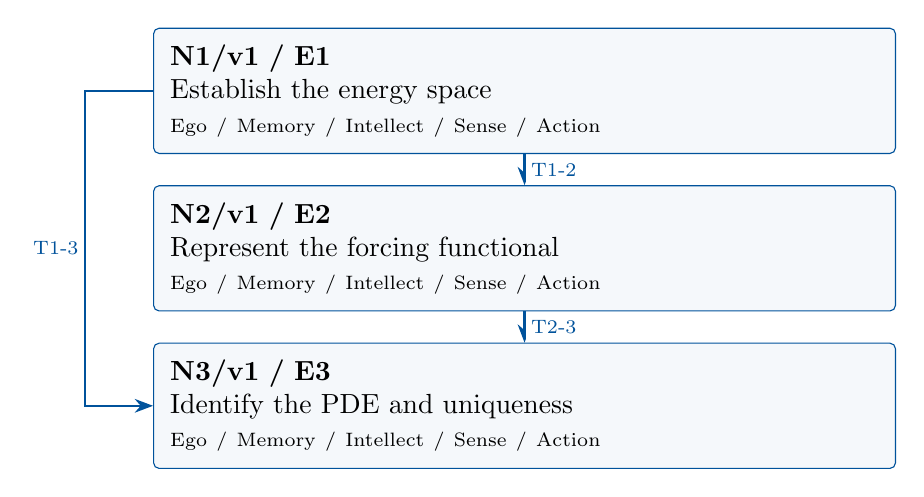
\begin{tikzpicture}[>=Stealth,x=1cm,y=1cm]

\node[mmnode,text width=9cm,minimum height=1.25cm] (N1) at (0,0.0) {\textbf{N1/v1 / E1}\\Establish the energy space\\{\scriptsize Ego / Memory / Intellect / Sense / Action}};

\node[mmnode,text width=9cm,minimum height=1.25cm] (N2) at (0,-2.0) {\textbf{N2/v1 / E2}\\Represent the forcing functional\\{\scriptsize Ego / Memory / Intellect / Sense / Action}};

\node[mmnode,text width=9cm,minimum height=1.25cm] (N3) at (0,-4.0) {\textbf{N3/v1 / E3}\\Identify the PDE and uniqueness\\{\scriptsize Ego / Memory / Intellect / Sense / Action}};

\draw[mmproof] (N1.south) -- node[mmnote,right] {T1-2} (N2.north);

\draw[mmproof] (N1.west) -- (-5.58,0) -- node[mmnote,left] {T1-3} (-5.58,-4) -- (N3.west);

\draw[mmproof] (N2.south) -- node[mmnote,right] {T2-3} (N3.north);

\end{tikzpicture}\end{center}

Each box is one mathematical agent containing all five faculties. Blue
arrows carry the versioned exports listed below. The layout gives a
reading order; only drawn arrows assert dependencies. Diagnostic repair
is separate from the proof DAG.

\subsection{Versioned evidence-transfer ledger}

\begingroup\small\linespread{1.05}\selectfont

\Needspace{5\baselineskip}\field{T1-2: N1/E1/v1 to N2}{\(\|v\|_2\le L\|\nabla v\|_2\) on \(H_0^1\), and
\(a(u,v)=\int\nabla u\cdot\nabla v\) is a complete inner product there.}

\field{Receiving activity}{N2.1}

\field{Compatibility}{E1/v1 and \(\ell(v)=\int_\Omega fv\). Check: The functional is defined
on equivalence classes and bounded in the gradient norm, not merely in
the \(L^2\) norm.}

\Needspace{5\baselineskip}\field{T1-3: N1/E1/v1 to N3}{\(\|v\|_2\le L\|\nabla v\|_2\) on \(H_0^1\), and
\(a(u,v)=\int\nabla u\cdot\nabla v\) is a complete inner product there.}

\field{Receiving activity}{N3.2}

\field{Compatibility}{E2/v1 and the definition of distributional Laplacian. Check: The
conclusion is weak existence; no \(C^2\) regularity or pointwise
boundary trace on a rough domain is inferred.}

\Needspace{5\baselineskip}\field{T2-3: N2/E2/v1 to N3}{There exists \(u\in H_0^1\) with \(a(u,v)=\ell(v)\) for all \(v\), and
\(\|\nabla u\|_2\le L\|f\|_2\).}

\field{Receiving activity}{N3.1}

\field{Compatibility}{E2/v1 and the definition of distributional Laplacian. Check: The
conclusion is weak existence; no \(C^2\) regularity or pointwise
boundary trace on a rough domain is inferred.}

\endgroup

\clearpage\section{Agent roles and five-faculty activities}\begingroup\small\linespread{1.05}\selectfont\setlist{itemsep=1pt,topsep=2pt}

\subsection{N1/v1: Establish the energy space}

\field{Object and role}{Integrate along one coordinate to prove Poincaré, then use density and
equivalent norms. \textbf{Local obligation:}
\(\|v\|_2\le L\|\nabla v\|_2\) on \(H_0^1\), and
\(a(u,v)=\int\nabla u\cdot\nabla v\) is a complete inner product there.}

\field{Inputs}{A cube \(Q\) of side \(L\) containing \(\Omega\) and smooth compactly
supported test functions extended by zero to \(Q\).}

\mmfaculty{E}{Ego}{Publish E1/v1 only after establishing this obligation:
\(\|v\|_2\le L\|\nabla v\|_2\) on \(H_0^1\), and
\(a(u,v)=\int\nabla u\cdot\nabla v\) is a complete inner product there.}

\mmfaculty{M}{Memory}{A cube \(Q\) of side \(L\) containing \(\Omega\) and smooth compactly
supported test functions extended by zero to \(Q\). Retain the stated
assumptions and import versions.}

\mmfaculty{I}{Intellect}{Integrate along one coordinate to prove Poincaré, then use density and
equivalent norms.}

\mmfaculty{S}{Sense}{Zero extension is used first only for compactly supported smooth
functions; the general inequality follows by the defining closure.}

\mmfaculty{A}{Action}{Carry out activities N1.1--N1.2 below, retaining each calculation and
construction as evidence.}

\smallskip\noindent\textbf{Numbered mathematical activities}

\begin{enumerate}[label=N1.\arabic*,leftmargin=3.4em]

\item After translating the cube, take \(Q=(0,L)^d\). For
\(v\in C_c^\infty(\Omega)\) extended by zero,
\(v(x_1,x')=\int_0^{x_1}\partial_1v(s,x')\,ds\). Cauchy--Schwarz gives
\(|v(x_1,x')|^2\le L\int_0^L|\partial_1v(s,x')|^2ds\). Integrate over
\(x_1\) and \(x'\) to obtain
\(\|v\|_2^2\le L^2\|\partial_1v\|_2^2\le L^2\|\nabla v\|_2^2\).

\item Approximate any \(v\in H_0^1\) by such smooth functions in the \(H^1\)
norm. Passing to the norm limit preserves the inequality. Therefore
\(\|\nabla v\|_2=0\) forces \(v=0\), and the gradient norm is equivalent
to the complete \(H^1\) norm on its closed subspace \(H_0^1\). A
gradient-Cauchy sequence is \(H^1\)-Cauchy by the inequality and
converges in both norms. Thus \(a\) is a Hilbert inner product.

\end{enumerate}

\field{Export E1/v1}{\(\|v\|_2\le L\|\nabla v\|_2\) on \(H_0^1\), and
\(a(u,v)=\int\nabla u\cdot\nabla v\) is a complete inner product there.}

\field{Acceptance gate}{Zero extension is used first only for compactly supported smooth
functions; the general inequality follows by the defining closure.}

\field{Targeted repair}{If the gradient seminorm is called a norm without justification, prove
Poincaré first; constants are not automatically excluded in other
Sobolev spaces. Withhold this export and recheck its descendants after a
versioned correction.}

\clearpage

\subsection{N2/v1: Represent the forcing functional}

\field{Object and role}{Bound the forcing in the energy norm and apply the declared Hilbert
representation theorem. \textbf{Local obligation:} There exists
\(u\in H_0^1\) with \(a(u,v)=\ell(v)\) for all \(v\), and
\(\|\nabla u\|_2\le L\|f\|_2\).}

\field{Inputs}{E1/v1 and \(\ell(v)=\int_\Omega fv\). Incoming proof exports: E1/v1 at
N2.1.}

\mmfaculty{E}{Ego}{Publish E2/v1 only after establishing this obligation: There exists
\(u\in H_0^1\) with \(a(u,v)=\ell(v)\) for all \(v\), and
\(\|\nabla u\|_2\le L\|f\|_2\).}

\mmfaculty{M}{Memory}{E1/v1 and \(\ell(v)=\int_\Omega fv\). Incoming proof exports: E1/v1 at
N2.1. Retain the stated assumptions and import versions.}

\mmfaculty{I}{Intellect}{Bound the forcing in the energy norm and apply the declared Hilbert
representation theorem.}

\mmfaculty{S}{Sense}{The functional is defined on equivalence classes and bounded in the
gradient norm, not merely in the \(L^2\) norm.}

\mmfaculty{A}{Action}{Carry out activities N2.1--N2.2 below, retaining each calculation and
construction as evidence.}

\smallskip\noindent\textbf{Numbered mathematical activities}

\begin{enumerate}[label=N2.\arabic*,leftmargin=3.4em]

\item Cauchy--Schwarz and E1 give
\(|\ell(v)|\le\|f\|_2\|v\|_2\le L\|f\|_2\|\nabla v\|_2\). Thus \(\ell\)
is a bounded linear functional on the real Hilbert space with inner
product \(a\).

\item Apply FA-03 to obtain a unique representing vector \(u\) with
\(\ell(v)=a(v,u)=a(u,v)\), since the form is symmetric. The norm
equality in Riesz yields \(\|\nabla u\|_2=\|\ell\|\le L\|f\|_2\). This
is exactly the asserted variational equation.

\end{enumerate}

\field{Export E2/v1}{There exists \(u\in H_0^1\) with \(a(u,v)=\ell(v)\) for all \(v\), and
\(\|\nabla u\|_2\le L\|f\|_2\).}

\field{Acceptance gate}{The functional is defined on equivalence classes and bounded in the
gradient norm, not merely in the \(L^2\) norm.}

\field{Targeted repair}{If the functional is represented using the usual \(H^1\) inner product,
change to \(a\); otherwise an unwanted zeroth-order term appears.
Withhold this export and recheck its descendants after a versioned
correction.}

\clearpage

\subsection{N3/v1: Identify the PDE and uniqueness}

\field{Object and role}{Test against compactly supported smooth functions and against the
difference of two proposed solutions. \textbf{Local obligation:} The
vector \(u\) solves \(-\Delta u=f\) in distributions and is the unique
stated weak solution.}

\field{Inputs}{E2/v1 and the definition of distributional Laplacian. Incoming proof
exports: E1/v1 at N3.2, E2/v1 at N3.1.}

\mmfaculty{E}{Ego}{Publish E3/v1 only after establishing this obligation: The vector \(u\)
solves \(-\Delta u=f\) in distributions and is the unique stated weak
solution.}

\mmfaculty{M}{Memory}{E2/v1 and the definition of distributional Laplacian. Incoming proof
exports: E1/v1 at N3.2, E2/v1 at N3.1. Retain the stated assumptions and
import versions.}

\mmfaculty{I}{Intellect}{Test against compactly supported smooth functions and against the
difference of two proposed solutions.}

\mmfaculty{S}{Sense}{The conclusion is weak existence; no \(C^2\) regularity or pointwise
boundary trace on a rough domain is inferred.}

\mmfaculty{A}{Action}{Carry out activities N3.1--N3.2 below, retaining each calculation and
construction as evidence.}

\smallskip\noindent\textbf{Numbered mathematical activities}

\begin{enumerate}[label=N3.\arabic*,leftmargin=3.4em]

\item For \(\varphi\in C_c^\infty(\Omega)\subset H_0^1\), the distribution
\(-\Delta u\) acts by \(\int\nabla u\cdot\nabla\varphi\). The
variational identity equals \(\int f\varphi\), proving the
distributional equation. Membership in \(H_0^1\) is the specified
homogeneous boundary condition.

\item If \(u_1,u_2\) solve the equation, their difference \(w\) satisfies
\(a(w,v)=0\) for every \(v\in H_0^1\). Choosing \(v=w\) gives
\(\|\nabla w\|_2^2=0\), and E1 gives \(w=0\). This independently
verifies uniqueness and closes the problem.

\end{enumerate}

\field{Export E3/v1}{The vector \(u\) solves \(-\Delta u=f\) in distributions and is the
unique stated weak solution.}

\field{Acceptance gate}{The conclusion is weak existence; no \(C^2\) regularity or pointwise
boundary trace on a rough domain is inferred.}

\field{Targeted repair}{If a weak solution is promoted to a classical one, remove that
unsupported conclusion or supply a separate regularity theorem with its
required domain assumptions. Withhold this export and recheck its
descendants after a versioned correction.}

\endgroup\clearpage\section{Continuous mathematical proof}\label{sec:proof}

\subsection{N1 --- Establish the energy
space}\label{n1-establish-the-energy-space}

\begin{enumerate}
\def\labelenumi{\arabic{enumi}.}
\item
  \textbf{N1.1.} After translating the cube, take \(Q=(0,L)^d\). For
  \(v\in C_c^\infty(\Omega)\) extended by zero,
  \(v(x_1,x')=\int_0^{x_1}\partial_1v(s,x')\,ds\). Cauchy--Schwarz gives
  \(|v(x_1,x')|^2\le L\int_0^L|\partial_1v(s,x')|^2ds\). Integrate over
  \(x_1\) and \(x'\) to obtain
  \(\|v\|_2^2\le L^2\|\partial_1v\|_2^2\le L^2\|\nabla v\|_2^2\).
\item
  \textbf{N1.2.} Approximate any \(v\in H_0^1\) by such smooth functions
  in the \(H^1\) norm. Passing to the norm limit preserves the
  inequality. Therefore \(\|\nabla v\|_2=0\) forces \(v=0\), and the
  gradient norm is equivalent to the complete \(H^1\) norm on its closed
  subspace \(H_0^1\). A gradient-Cauchy sequence is \(H^1\)-Cauchy by
  the inequality and converges in both norms. Thus \(a\) is a Hilbert
  inner product.
\end{enumerate}

\subsection{N2 --- Represent the forcing
functional}\label{n2-represent-the-forcing-functional}

\begin{enumerate}
\def\labelenumi{\arabic{enumi}.}
\item
  \textbf{N2.1.} Cauchy--Schwarz and E1 give
  \(|\ell(v)|\le\|f\|_2\|v\|_2\le L\|f\|_2\|\nabla v\|_2\). Thus
  \(\ell\) is a bounded linear functional on the real Hilbert space with
  inner product \(a\).
\item
  \textbf{N2.2.} Apply FA-03 to obtain a unique representing vector
  \(u\) with \(\ell(v)=a(v,u)=a(u,v)\), since the form is symmetric. The
  norm equality in Riesz yields \(\|\nabla u\|_2=\|\ell\|\le L\|f\|_2\).
  This is exactly the asserted variational equation.
\end{enumerate}

\subsection{N3 --- Identify the PDE and
uniqueness}\label{n3-identify-the-pde-and-uniqueness}

\begin{enumerate}
\def\labelenumi{\arabic{enumi}.}
\item
  \textbf{N3.1.} For \(\varphi\in C_c^\infty(\Omega)\subset H_0^1\), the
  distribution \(-\Delta u\) acts by \(\int\nabla u\cdot\nabla\varphi\).
  The variational identity equals \(\int f\varphi\), proving the
  distributional equation. Membership in \(H_0^1\) is the specified
  homogeneous boundary condition.
\item
  \textbf{N3.2.} If \(u_1,u_2\) solve the equation, their difference
  \(w\) satisfies \(a(w,v)=0\) for every \(v\in H_0^1\). Choosing
  \(v=w\) gives \(\|\nabla w\|_2^2=0\), and E1 gives \(w=0\). This
  independently verifies uniqueness and closes the problem.
\end{enumerate}

\hfill$\square$

\section{Worked orchestration}

On \(\Omega=(0,1)\) with \(f=1\), let \(u(x)=x(1-x)/2\). It belongs to
\(H_0^1\): smooth cutoffs near the endpoints converge in \(H^1\), since
\(u\) vanishes linearly there and the cutoff-derivative errors are
supported on intervals of vanishing length. It satisfies \(-u''=1\).
Integration by parts against smooth compactly supported \(v\) gives
\(\int u'v'=\int v\), and density extends this to all \(H_0^1\). Its
energy norm is \(\|u'\|_2=1/\sqrt{12}\le1=L\|f\|_2\).

\subsection{Boundary and hypothesis audit}

On \(H^1(\Omega)\) instead of \(H_0^1\), a nonzero constant has zero
gradient, so the energy form is not an inner product. Testing the same
proposed equation with \(v=1\) would require \(\int f=0\), a
compatibility condition absent from the Dirichlet theorem. Changing the
space changes the problem.

\section{Illustrative failure and repair}

The following is an authored diagnostic scenario. Changed assumptions
define a new contract; they do not retroactively prove the original
statement.

\subsection{Rejected argument, diagnosis, and correction}
\textbf{Rejected N1 export:} the gradient norm is complete and positive
on all \(H^1\). \textbf{Sense:} nonzero constants have norm zero in that
seminorm. \textbf{Repair:} retain \(H_0^1\) and the explicit Poincaré
estimate before applying Riesz. The original weak Dirichlet target is
unchanged. Recheck the forcing bound, representation, and uniqueness
downstream.

\subsection{Publication and reuse}
The corrected export retains its explicit assumptions. A hypothetical
revision receives a new version, and each consuming activity is
rechecked; this scenario is not a recorded runtime event. \textbf{Next
direction:} Develop Lax--Milgram for nonsymmetric coercive forms, or
establish additional regularity under smoother domain and forcing
assumptions.

\par\medskip\begingroup\small\linespread{1.0}\selectfont\noindent\textbf{Provenance.} This authored proof is complete relative to its declared imports. Reuse
each export with its assumptions, proof, and version. The original
Markdown remains available for comparison.
\par\endgroup

\par\smallskip\begingroup\small\linespread{1.0}\selectfont\noindent\textbf{Further reading.} \href{https://math.stanford.edu/~lms/lecs-on-pde.pdf}{Leon Simon,
Lectures on PDE}, for elliptic, weak, and parabolic methods. Classical
calculus and the explicitly stated Hilbert-space imports are used below;
the displayed PDE arguments are developed in full.\par\endgroup

\end{document}
